\chapter{Beschreibung des Messverfahrens}
\label{sec:measurement}
Ein vereinfachtes Schaltbild eines Eingangs-/Ausgangs-Pin des ATmega wird in Abbildung~\ref{fig:port} gezeigt.
Der Schalter PUD schaltet die Versorgung für alle \inquotes{Pull Up}-Widerstände des ATmega ab.
Mit dem Schalter DD kann der Ausgang abgeschaltet werden, der Eingang funktioniert sowohl im Ausgabe- wie im
Eingabe-Modus. Im Eingabe-Modus wird mit dem Ausgabewert (PORT) der \inquotes{Pull Up}-Widerstand des Eingangs mit geschaltet.
Die beiden Schalter PORT und DD können nicht gleichzeitig, sondern nur nacheinander geschaltet werden.
Weil beim Umschalten der \inquotes{Pull Up}-Widerstand die Messung stören könnte, bevorzuge ich die komplette
Abschaltung aller \inquotes{Pull Up}-Widerstände mit dem PUD-Schalter.
Natürlich sind die Schalter elektronisch und die Widerstände \(19\Omega\) und \(22\Omega\) sind angenäherte Werte.
\begin{figure}[H]
\centering
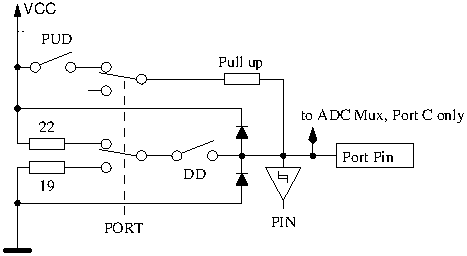
\includegraphics[width=.8\textwidth]{../FIG/port.pdf}
\caption{Vereinfachtes Schaltbild jedes ATmega-Portpins}
\label{fig:port}
\end{figure}

Jeder der drei Testpins Ihres TransistorTesters wird aus drei ATmega-Portpins gebildet,
was im vereinfachten Schaltbild des Testpins TP2 (mittlerer der drei Pins) in Abbildung~\ref{fig:terminal} gezeigt wird.

\begin{figure}[H]
\centering
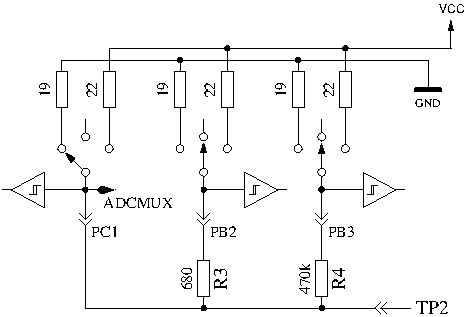
\includegraphics[width=.8\textwidth]{../FIG/terminal.pdf}
\caption{Vereinfachtes Schaltbild des Testpins TP2}
\label{fig:terminal}
\end{figure}

Jeder Testpin (Messport) kann als digitaler oder analoger Eingang benutzt werden.
Diese Mess\-fähig\-keit ist un\-abhän\-gig von der Verwendung des Ports als Ausgang.
Jeder Testpin kann als Ausgang verwendet werden und in diesem Zustand mit GND (\(0V\)) oder VCC (\(5V\)) verbunden werden,
oder er kann über die Widerstände (\(680\Omega\) oder \(470k\Omega\)) mit entweder GND oder VCC verbunden werden.
Tabelle \ref{tab:case} zeigt alle denkbaren Messmöglichkeiten.
Beachten Sie, dass der positive Zustand durch direktes Verbinden mit VCC (Port C) oder
durch Verbinden mit dem \(680\Omega\) Widerstand mit VCC (Port B) erreicht werden kann.
Die gleiche Möglichkeit hat der negative Zustand des Testpins zu der GND-Seite.
Der Test-Zustand meint, dass der Pin offen sein kann (Eingang), verbunden über den \(470k\Omega\)-Widerstand
mit VCC oder GND, oder der Pin kann über den \(680\Omega\)-Widerstand mit VCC oder GND verbunden sein.

\begin{table}[H]
  \begin{center}
    \begin{tabular}{| l | c | c | c |}
    \hline
      & Zustand Pin 1 & Zustand Pin 2 & Zustand Pin 3 \\
    \hline
   1. & positiv    &  negativ   &  test \\
   2. & positiv    &  test      & negativ \\
   3. & test       &  negativ   & positiv \\
   4. & test       &  positiv   & negativ \\
   5. & negativ    &  test      & positiv \\
   6. & negativ    &  positiv   &  test  \\
    \hline
    \end{tabular}
  \end{center}
  \caption{alle Messmöglichkeiten}
  \label{tab:case} 
\end{table}

Wenn die Kondensatormessung des Testers konfiguriert ist, versucht der Tester vor allen Messungen erst einmal,
die Kondensatoren an allen Anschlusspins zu entladen. Wenn das nicht gelingt, also die Restspannung zu hoch bleibt,
wird das Entladen nach etwa 12 Sekunden mit der Meldung \inquotes{Cell!} abgebrochen. Dies kann auch dann vorkommen, wenn
gar kein Kondensator angeschlossen ist. Die Ursache kann in diesem Fall sein, dass die Entlade-Grenzspannung für diesen
ATmega zu niedrig gewählt ist. Man kann eine höhere Restspannung mit der Makefile-Option CAP\_EMPTY\_LEVEL wählen.
